% Provenance (never printed): see sources/outline_sources.md (Year 3: the heat
% equation, half-space and plate cooling models, heat flow against age,
% continental geotherms, thermal subsidence). Brief: sources/book5/BRIEFS.md,
% ch. 5. Curves from figdata/bachelor-3/plate_cooling.py (models; Seton et al.
% 2020 age grid and ETOPO1, read only) and continental_geotherm.py.
% Exercise and problem values in the Book 5 scratch calculator calc/ch05.py.
\chapter{स्थलमंडल के ऊष्मीय मॉडल}\label{ch:b3:lithosphere-thermal-models}

मध्य-महासागरीय कटक से दूर जाने पर महासागरीय तल गहरा होता जाता है: अक्ष पर लगभग
\qty{2.5}{km}, और सबसे पुराने महासागरीय तल के नीचे \qty{5}{km} से अधिक।
प्लेट में कुछ जोड़ा नहीं गया है और न उससे कुछ हटाया गया है; वह केवल
ठंडी हुई, सिकुड़ी और धँस गई है। महासागरीय तल अपने नीचे की प्लेट का तापमापी है,
और उसके अवसाद में धँसाया गया ऊष्मा-प्रवाह संवेदक ऊपर से वही शीतलन पढ़ता है।
यह अध्याय प्लेट के शीतलन को दो तरीकों से हल करता है: अर्ध-समष्टि के रूप में
और परिमित मोटाई की प्लेट के रूप में, दोनों की तुलना वास्तविक महासागरीय तल की गहराई
और उसके ऊष्मा-प्रवाह से करता है, फिर महाद्वीपों की ओर मुड़ता है,
जिनकी ऊष्मा का कुछ भाग उनकी अपनी भूपर्पटी से आता है।
% ledger: ps77:depth-age

\begin{recall}
ऊष्मा के लिए विसरण समीकरण, $\partial T/\partial t = \kappa\nabla^2T$,
जिसमें तापीय चालकता $k$ और तापीय विसरणता $\kappa =
k/(\rho c)$, भौतिकी की पुस्तकों में है; फ़ूरिये श्रेणी और त्रुटि-फलन
$\operatorname{erf}x = (2/\sqrt\pi)\int_0^xe^{-u^2}\,\mathrm du$ गणित की पुस्तकों के
विश्वविद्यालयी खंडों में हैं। ऊष्मा-प्रवाह, रेडियोजनित ऊष्मा-उत्पादन,
जियोथर्म, चालन-काल $L^2/\kappa$, ऊष्मीय
सीमा-परत और ऊष्मीय स्थलमंडल पुस्तक 3 (स्नातक वर्ष 1) में परिभाषित हुए थे,
पृथ्वी के ऊष्मा-बजट वाले अध्याय में; समस्थिति उसके समस्थिति वाले
और गुरुत्व विसंगतियों वाले अध्याय में; गहराई–आयु नियम $d = d_r + C\sqrt t$
दरार, कटक और निष्क्रिय किनारों वाले अध्याय में सिद्ध हुआ था, इस अध्याय द्वारा
व्युत्पन्न तापमान-रूपरेखा को मानते हुए। द्रोणियों का खिंचाव प्रतिरूप, दरार-उत्तर
अवधसान और ऊष्मीय समय-स्थिरांक पुस्तक 4 (स्नातक वर्ष 2) में हैं, उसके
अवसादी द्रोणी वाले अध्याय में।
\end{recall}

\section{चालन, अभिवहन और उनका अनुपात}

स्थलमंडल में ऊष्मा दो तरह से चलती है: वह तापमान-प्रवणता की दिशा में विसरित होती है,
और गतिमान चट्टान द्वारा वहन की जाती है, जैसे कटक से निकलती प्लेट, अपरदित
पर्वत का उत्थान, मैग्मा का ऊपर उठना। कौन-सा तरीका प्रबल होता है, यह एक ही
संख्या पर निर्भर करता है।

\begin{definition}[ऊष्मीय पेक्ले संख्या]\label{def:b3:lithosphere-thermal-models:peclet}
चाल $u$ से, लंबाई $L$ के आर-पार गतिमान चट्टान के लिए, \emph{ऊष्मीय पेक्ले
संख्या}\index{ऊष्मीय पेक्ले संख्या} होती है
\[
  \mathrm{Pe} = \frac{uL}{\kappa},
\]
यह चालन-काल $L^2/\kappa$ और अभिवहन-काल $L/u$ का अनुपात है।
जहाँ $\mathrm{Pe} \gg 1$ हो वहाँ अभिवहन प्रबल होता है, और जहाँ
$\mathrm{Pe} \ll 1$ हो वहाँ चालन प्रबल होता है।
\end{definition}

कटक से \qty{25}{mm/yr} पर निकलती एक प्लेट के लिए, \qty{95}{km} की दूरी पर
$\mathrm{Pe} \approx 94$ होता है, जब $\kappa = \qty{0.8e-6}{m^2.s^{-1}}$ हो:
ऊष्मा प्लेट द्वारा पार्श्व दिशा में उसके विसरण की तुलना में कहीं अधिक तेज़ी से वहन होती है।
इसलिए प्लेट का प्रत्येक ऊर्ध्वाधर स्तंभ मानो अकेला हो, इस प्रकार ठंडा होता है, ऊर्ध्वाधर
चालन द्वारा ठंडे महासागरीय तल तक, जहाँ आयु $t$ उस समय को दर्शाती है जब से वह
अक्ष से निकला था। इससे द्वि-आयामी समस्या गहराई और
समय की एक समस्या में बदल जाती है।

\section{शीतलन अर्ध-समष्टि}

\begin{definition}[अर्ध-समष्टि शीतलन मॉडल]\label{def:b3:lithosphere-thermal-models:half-space}
\emph{अर्ध-समष्टि शीतलन मॉडल}\index{अर्ध-समष्टि शीतलन मॉडल} महासागरीय स्थलमंडल के लिए
प्रत्येक स्तंभ को एकसमान विसरणता वाला एक अर्ध-समष्टि $z \ge 0$ मानता है, जो कटक-अक्ष
से निकलते समय प्रावार के एकसमान तापमान $T_m$ पर होता है, और जिसकी सतह उसी समय से
महासागरीय तल के तापमान $T_0$ पर स्थिर रखी जाती है, बिना ऊष्मा-उत्पादन और बिना
निचली सीमा के।
\end{definition}

\begin{theorem}[त्रुटि-फलन जियोथर्म]\label{thm:b3:lithosphere-thermal-models:erf}
\omterm{def:b3:lithosphere-thermal-models:half-space}{अर्ध-समष्टि शीतलन मॉडल} में महासागरीय तल के नीचे गहराई $z$ पर,
जिसकी आयु $t$ है, तापमान इस प्रकार है:
\[
  T(z, t) = T_0 + (T_m - T_0)\operatorname{erf}\frac{z}{2\sqrt{\kappa t}} .
\]
यह \emph{त्रुटि-फलन जियोथर्म}\index{त्रुटि-फलन जियोथर्म} है।
\end{theorem}

\begin{proof}
मान लीजिए $\theta = (T - T_0)/(T_m - T_0)$; यह $\partial\theta/\partial t =
\kappa\,\partial^2\theta/\partial z^2$ को संतुष्ट करता है, जिसमें $\theta(z, 0) = 1$ है, जहाँ $z > 0$ और
$\theta(0, t) = 0$ है, जहाँ $t > 0$। इस समस्या का अपना कोई लंबाई-पैमाना नहीं है:
यदि $\theta(z, t)$ एक हल है, तो $\theta(\lambda z, \lambda^2t)$ भी हर
$\lambda > 0$ के लिए हल है, उन्हीं आरंभिक और सीमा-मानों के साथ; हल
एकमात्र है, इसलिए $\theta$ $z$ और $t$ पर केवल $\eta = z/(2\sqrt{\kappa
t})$ के माध्यम से निर्भर करता है। $\theta = f(\eta)$ लिखकर, $\partial\eta/\partial t = -\eta/(2t)$ और
$\partial\eta/\partial z = 1/(2\sqrt{\kappa t})$ लेकर,
\[
  -\frac{\eta}{2t}f'(\eta) = \kappa\,\frac{f''(\eta)}{4\kappa t},
  \qquad\text{अतः}\qquad f'' + 2\eta f' = 0 .
\]
अतः $f' = Ae^{-\eta^2}$ और $f = A\int_0^\eta e^{-u^2}\,\mathrm du + B$ होता है।
सतह-शर्त, $\eta = 0$ पर, $B = 0$ देती है; आरंभिक शर्त, जो
हर गहराई पर लागू होती है, जब $t \to 0$, अर्थात $\eta \to \infty$, वह
$A\sqrt\pi/2 = 1$ देती है। अतः $f = \operatorname{erf}\eta$ है।
\end{proof}

किसी दी गई गहराई पर तापमान केवल $z/\sqrt t$ पर निर्भर करता है: एक समतापरेखा
आयु के वर्गमूल के अनुपात में नीचे धँसती है, और \qty{40}{Myr} पर शीतल परत
\qty{10}{Myr} की तुलना में दोगुनी मोटी है। सतही ऊष्मा-प्रवाह अवकलन द्वारा प्राप्त होता है।

\begin{proposition}[ऊष्मा-प्रवाह--आयु संबंध]\label{prop:b3:lithosphere-thermal-models:heat-flow}
\omterm{def:b3:lithosphere-thermal-models:half-space}{अर्ध-समष्टि शीतलन मॉडल} में आयु $t$ के महासागरीय तल से होकर बहने वाला
ऊष्मा-प्रवाह इस प्रकार है:
\[
  q(t) = k\,\frac{\partial T}{\partial z}\Big|_{z=0}
  = \frac{k(T_m - T_0)}{\sqrt{\pi\kappa t}} = \frac{C_q}{\sqrt t} .
\]
\end{proposition}

\begin{proof}
$\partial\operatorname{erf}(z/2\sqrt{\kappa t})/\partial z = (2/\sqrt\pi)
e^{-z^2/4\kappa t}/(2\sqrt{\kappa t})$, जहाँ $z = 0$ पर $1/\sqrt{\pi\kappa
t}$ है।
\end{proof}

नीचे दिए प्लेट मॉडल के मानों के साथ ($k = \qty{3.1}{W.m^{-1}.K^{-1}}$,
$T_m - T_0 = \qty{1450}{K}$, $\kappa = \qty{0.8e-6}{m^2.s^{-1}}$), $C_q =
\qty{505}{mW.m^{-2}.Myr^{1/2}}$, विभिन्न अध्ययनों द्वारा वैश्विक मापों पर फ़िट किए गए 430 से
\qty{510}{mW.m^{-2}.Myr^{1/2}} तक के मानों के निकट है;
एक हालिया संकलन \num{490} को प्राथमिकता देता है। युवा महासागरीय भूपर्पटी पर मापा गया
ऊष्मा-प्रवाह, फिर भी, उससे निकलने वाली ऊष्मा को बहुत कम आँकता है:
दरारों वाली भूपर्पटी से होकर परिसंचारित समुद्री जल ऊष्मा का कुछ भाग दूर ले जाता है
गर्म सोतों के माध्यम से, संवेदकों की पहुँच से बाहर। पुरानी भूपर्पटी पर मापन
$1/\sqrt t$ का अनुसरण करते हैं, और पृथ्वी की ऊष्मा-हानि के अनुमान
\qty{66.5}{Myr} से कम आयु की भूपर्पटी पर मापनों की जगह $C_q/\sqrt t$ रखते हैं।
% ledger: honda04:gdh1, b2dd10:half-space, dd10b5:hydrothermal

पुस्तक 3 (स्नातक वर्ष 1) ने वही प्रोफ़ाइल गहराई पर, समस्थिति के माध्यम से, समाकलित करके
गहराई--आयु नियम प्राप्त किया, $d = d_r + C\sqrt t$, जिसमें $C = 2\rho_m\alpha(T_m -
T_0)\sqrt\kappa/\bigl(\sqrt\pi(\rho_m - \rho_w)\bigr)$ (नीचे का चित्र देखिए)।
इनके लिए $\rho_m = \qty{3300}{kg.m^{-3}}$, $\rho_w = \qty{1030}{kg.m^{-3}}$ और $\alpha =
\qty{3.1e-5}{K^{-1}}$, $C = \qty{370}{m.Myr^{-1/2}}$ प्राप्त होता है, जो
उत्तरी प्रशांत और उत्तरी अटलांटिक तलों पर फ़िट किए गए \qty{350}{m.Myr^{-1/2}} के मान की तुलना में
\qty{70}{Myr} से कम आयु वाले तलों पर तुलनीय है।
% ledger: ps77:depth-age

\begin{omfigure}
\begin{tikzpicture}[font=\small, x=1cm, y=1cm]
% schematic: two columns of equal mass above the compensation depth
\fill[blue!12] (0,0) rectangle (1.6,-1.2);
\fill[orange!35] (0,-1.2) rectangle (1.6,-5.6);
\fill[blue!12] (4.4,0) rectangle (6.6,-2.2);
\shade[top color=blue!35!gray!40, bottom color=orange!35] (4.4,-2.2) rectangle (6.6,-4.4);
\fill[orange!35] (4.4,-4.4) rectangle (6.6,-5.6);
\draw (0,0) rectangle (1.6,-5.6) (4.4,0) rectangle (6.6,-5.6);
\draw[densely dashed] (-0.6,-5.6) -- (7.2,-5.6) node[right, font=\scriptsize] {प्रतिपूर्ति गहराई};
\draw[thick] (0,-1.2) -- (1.6,-1.2) (4.4,-2.2) -- (6.6,-2.2);
\node[font=\scriptsize] at (0.8,-0.6) {जल};
\node[font=\scriptsize, align=center] at (0.8,-3.4) {प्रावार\\$T_m$ पर};
\node[font=\scriptsize] at (5.5,-1.1) {जल};
\node[font=\scriptsize, align=center] at (5.5,-3.3) {शीतल प्लेट\\$\rho_m(1 + \alpha\,\Delta T)$};
\node[font=\scriptsize, align=center] at (5.5,-5.0) {प्रावार};
\draw[<->] (-0.3,0) -- (-0.3,-1.2) node[midway, left, font=\scriptsize] {$d_r$};
\draw[<->] (6.9,0) -- (6.9,-2.2) node[midway, right, font=\scriptsize] {$d(t)$};
\node[above, font=\scriptsize] at (0.8,0.05) {कटक-अक्ष};
\node[above, font=\scriptsize] at (5.5,0.05) {आयु $t$ का तल};
\draw[gray] (-0.6,0) -- (7.2,0);
\end{tikzpicture}

\par\smallskip{\small शीतल प्लेट की समस्थिति: कटक पर का स्तंभ
और आयु $t$ वाले स्तंभ का, प्रतिपूर्ति गहराई के ऊपर, द्रव्यमान समान होता है।
शीतल होकर सघन हुई प्लेट धँसती है, और
उसके ऊपर का स्थान जल से भरता है।}\label{fig:b3:lithosphere-thermal-models:columns}
\end{omfigure}

\section{प्लेट मॉडल}

पुराना महासागरीय तल गहराना बंद कर देता है: उत्तरी प्रशांत और उत्तरी अटलांटिक में
गहराई $\sqrt t$ से 60 और \qty{80}{Myr} के बीच विचलित होती है, और ऊष्मा-प्रवाह
समतल हो जाता है। अर्ध-समष्टि सदा शीतल होता रहता है;
किसी प्रक्रिया को प्लेट के आधार को गर्म रखना होगा।
% ledger: parsons:plate-model

\begin{definition}[प्लेट शीतलन मॉडल]\label{def:b3:lithosphere-thermal-models:plate}
महासागरीय स्थलमंडल का \emph{प्लेट शीतलन मॉडल}\index{प्लेट शीतलन मॉडल} प्रत्येक स्तंभ को
एकसमान विसरणता वाली, $0 \le z \le L$ मोटाई की एक परत मानता है,
जो कटक को छोड़ते समय एकसमान तापमान $T_m$ पर होती है,
उसकी सतह $T_0$ पर रखी जाती है और उसी क्षण से उसका आधार $T_m$ पर रखा जाता है।
\end{definition}

\begin{theorem}[प्लेट-मॉडल तापमान श्रेणी]\label{thm:b3:lithosphere-thermal-models:plate-series}
\omterm{def:b3:lithosphere-thermal-models:plate}{प्लेट शीतलन मॉडल} में, $T_0 = 0$ लेकर,
\[
  T(z, t) = T_m\Bigl[\frac zL + \frac2\pi\sum_{n=1}^\infty\frac1n
  \sin\frac{n\pi z}{L}\,e^{-n^2t/\tau}\Bigr],\qquad
  \tau = \frac{L^2}{\pi^2\kappa} .
\]
यह \emph{प्लेट-मॉडल तापमान श्रेणी}\index{प्लेट-मॉडल तापमान श्रेणी} है।
\end{theorem}

\begin{proof}
$t \to \infty$ पर पहुँचने वाली स्थायी अवस्था रैखिक प्रोफ़ाइल $T_mz/L$ है।
विचलन $u = T - T_mz/L$ विसरण समीकरण का हल है, जिसकी सीमा-शर्त $u = 0$ है
$z = 0$ और $z = L$ पर, और आरंभिक मान $u(z, 0) = T_m(1 - z/L)$ है। चरों
का पृथक्करण करने पर, $u = Z(z)\Theta(t)$ से $Z''/Z = \Theta'/(\kappa\Theta) = -\mu^2$ प्राप्त होता है;
सीमा-शर्तें $Z = \sin(n\pi z/L)$ और $\mu = n\pi/L$ देती हैं, तथा
$\Theta = e^{-n^2\pi^2\kappa t/L^2} = e^{-n^2t/\tau}$ प्राप्त होता है। आरंभिक मान
गुणांक $b_n$ निश्चित करते हैं, जो $T_m(1 - z/L)$ की, $[0, L]$ पर, ज्या-श्रेणी के हैं:
\[
  b_n = \frac2L\int_0^LT_m\Bigl(1 - \frac zL\Bigr)\sin\frac{n\pi z}{L}\,\mathrm dz
  = \frac{2T_m}{n\pi},
\]
खंड-समाकलन द्वारा। मोडों का योग करने पर श्रेणी प्राप्त होती है।
\end{proof}

प्रत्येक मोड अपने समय-स्थिरांक $\tau/n^2$ के साथ क्षीण होता है: उच्चतर हार्मोनिक,
अर्थात आरंभिक चरण की सूक्ष्म संरचना, पहले विलीन हो जाते हैं, और $\tau$ कोटि के समय के बाद
केवल पहला बचता है। चरों के उसी पृथक्करण से ऊष्मा-प्रवाह प्राप्त होता है, और
ऊपर के चित्र के समस्थिति संतुलन द्वारा गहराई भी प्राप्त होती है।

\begin{proposition}[प्लेट मॉडल की गहराई और ऊष्मा-प्रवाह]\label{prop:b3:lithosphere-thermal-models:plate-depth}
\omterm{def:b3:lithosphere-thermal-models:plate}{प्लेट शीतलन मॉडल} में, गहराई--आयु नियम के
घनत्व और तापीय प्रसार के साथ,
\[
  q(t) = \frac{kT_m}{L}\Bigl[1 + 2\sum_{n=1}^\infty e^{-n^2t/\tau}\Bigr],\qquad
  d(t) = d_r + \frac{\rho_m\alpha T_mL}{2(\rho_m - \rho_w)}
  \Bigl[1 - \frac{8}{\pi^2}\sum_{n\ \text{विषम}}\frac{e^{-n^2t/\tau}}{n^2}\Bigr].
\]
$t \to \infty$ पर गहराई $d_r + \rho_m\alpha T_mL/\bigl(2(\rho_m -
\rho_w)\bigr)$ की ओर और ऊष्मा-प्रवाह $kT_m/L$ की ओर अग्रसर होते हैं, दोनों
घातांकीय रूप से, समय-स्थिरांक $\tau$ के साथ।
\end{proposition}

\begin{proof}
श्रेणी का $z = 0$ पर अवकलन करने से $\partial T/\partial z = (T_m/L)[1 +
2\sum e^{-n^2t/\tau}]$। गहराई के लिए समस्थिति संतुलन $(\rho_m -
\rho_w)(d - d_r) = \rho_m\alpha\int_0^L(T_m - T)\,\mathrm dz$ देता है। रैखिक भाग
$T_mL/2$ का योगदान देता है; प्रत्येक विधा का योगदान $-(2T_m/n\pi)e^{-n^2t/\tau}
\int_0^L\sin(n\pi z/L)\,\mathrm dz = -(2T_m/n\pi)(L/n\pi)(1 - \cos n\pi)
e^{-n^2t/\tau}$, जो सम $n$ के लिए शून्य है और $-(4T_mL/n^2\pi^2)
e^{-n^2t/\tau}$ विषम $n$ के लिए होता है। $T_mL/2$ निकालने पर कोष्ठक प्राप्त होता है। $t = 0$ पर
वह शून्य हो जाता है, क्योंकि $\sum_{n\ \text{विषम}}1/n^2 = \pi^2/8$।
\end{proof}

वैश्विक गहराइयों और ऊष्मा-प्रवाहों से सर्वोत्तम मेल खाने वाले प्लेट मॉडल में प्लेट की
मोटाई \qty{95}{km}, आधार \qty{1450}{\celsius} पर, $\alpha =
\qty{3.1e-5}{K^{-1}}$ और $k = \qty{3.1}{W.m^{-1}.K^{-1}}$, पतली और गर्म
पहले के \qty{125}{km} और \qty{1350}{\celsius} की तुलना में है। $\kappa =
\qty{0.8e-6}{m^2.s^{-1}}$, $\tau = \qty{36.2}{Myr}$ मानने पर; गहराई
$2500 + 3104 = \qty{5604}{m}$ पर स्थिर हो जाती है और ऊष्मा-प्रवाह \qty{47}{mW.m^{-2}} पर। युवा
तल दोनों मॉडलों में अंतर नहीं बता सकता: \qty{2}{Myr} पर उनमें एक मीटर से कम का
अंतर है, \qty{44}{Myr} पर \qty{100}{m} का। भूकंप-विज्ञान भी मिलता-जुलता
उत्तर देता है: प्रशांत महासागर की रैले तरंगें उन शीतलन प्लेटों से सर्वोत्तम रूप से समंजित होती हैं, जिनकी
स्पर्शोन्मुख मोटाई 85 से \qty{95}{km} है।
% ledger: honda04:gdh1, ps77:depth-age, fischer:lithosphere

\begin{omfigure}
\begin{tikzpicture}
\begin{groupplot}[group style={group size=1 by 2, vertical sep=2.3cm},
  omrecord, width=0.86\linewidth, height=0.42\linewidth, xmin=0, xmax=160,
  xlabel={समुद्री तल की आयु (Myr)}]
\nextgroupplot[omdepth, ylabel={गहराई (km)}, ymin=0, ymax=130,
  title={(क) समतापी रेखाएँ, प्रत्येक \qty{200}{\celsius} पर}, title style={font=\small},
  legend style={font=\scriptsize, at={(0.01,0.03)}, anchor=south west}]
% computed in figdata/bachelor-3/plate_cooling.py; ledger: honda04:gdh1
\addplot[omDef, thick] table[x=t, y=hs200] {figdata/out/bachelor-3-plate_cooling-isotherms.dat};
\addlegendentry{अर्ध-समष्टि}
\addplot[red!70!black, thick, densely dashed] table[x=t, y=pl200] {figdata/out/bachelor-3-plate_cooling-isotherms.dat};
\addlegendentry{प्लेट, $L = \qty{95}{km}$}
\foreach \lev in {400,600,800,1000,1200,1400} {
  \addplot[omDef, thick, forget plot] table[x=t, y=hs\lev] {figdata/out/bachelor-3-plate_cooling-isotherms.dat};
  \addplot[red!70!black, thick, densely dashed, forget plot] table[x=t, y=pl\lev] {figdata/out/bachelor-3-plate_cooling-isotherms.dat};
}
\draw[gray] (axis cs:0,95) -- (axis cs:160,95);
\node[font=\scriptsize, anchor=north] at (axis cs:68,96) {प्लेट का आधार};
\node[font=\scriptsize, fill=white, inner sep=1pt] at (axis cs:150,14) {200};
\node[font=\scriptsize, fill=white, inner sep=1pt] at (axis cs:28,38.2) {1000};
\node[font=\scriptsize, fill=white, inner sep=1pt] at (axis cs:22,70.4) {1400};
\nextgroupplot[ylabel={ऊष्मा-प्रवाह (\unit{mW.m^{-2}})}, ymin=0, ymax=300,
  title={(ख) ऊष्मा-प्रवाह}, title style={font=\small},
  legend style={font=\scriptsize, at={(0.98,0.97)}, anchor=north east}]
\addplot[omDef, thick] table[x=t, y=hs] {figdata/out/bachelor-3-plate_cooling-heat.dat};
\addlegendentry{अर्ध-समष्टि}
\addplot[red!70!black, thick, densely dashed] table[x=t, y=pl] {figdata/out/bachelor-3-plate_cooling-heat.dat};
\addlegendentry{प्लेट}
\end{groupplot}
\end{tikzpicture}

\par\smallskip{\small पाठ के मापदंडों वाले दो शीतलन मॉडल।
(क) समतापी रेखाओं की गहराई \qty{200}{\celsius} (ऊपर) से
\qty{1400}{\celsius} (नीचे) तक: अर्ध-समष्टि की समतापी रेखाएँ
$\sqrt t$ के अनुसार नीचे धँसती रहती हैं, जबकि प्लेट की रेखाएँ रुक जाती हैं जब परिच्छेदिका रैखिक हो जाती है। (ख) सतही
ऊष्मा-प्रवाह: प्लेट मॉडल \qty{47}{mW.m^{-2}} पर स्थिर हो जाता है, अर्ध-समष्टि
$1/\sqrt t$ के अनुसार घटता है।}\label{fig:b3:lithosphere-thermal-models:isotherms}
\end{omfigure}

वास्तविक महासागरीय तल को इसी ग्राफ़ पर रखा जा सकता है (नीचे का चित्र)। अक्षांश और देशांतर के एक-एक अंश का प्रत्येक खाना,
जिसकी आयु ज्ञात है, उसे अपनी आयु और
अपनी गहराई पर रखा जाता है; प्रत्येक पाँच-मिलियन-वर्षीय वर्ग की माध्यिका आयु के साथ बढ़ती है, जैसा मॉडल
पहले \qty{40}{Myr} तक कहते हैं, परंतु प्रेक्षित तल दोनों मॉडलों से
उथला है, और आयु के साथ यह अधिकाधिक ऐसा होता है। कुछ भी सुधारा नहीं गया है: पुराना तल
अवसाद की मोटी परत ढोता है, जो पुराने उत्तरी
अटलांटिक में एक किलोमीटर से अधिक है; यह उसे भारित करती है और उसका ऊपरी भाग ऊँचा कर देती है, और पुराने तल को
समुद्री पर्वत, ज्वालामुखीय पठार और हॉटस्पॉटों के उभार एकत्र करने का समय मिल चुका है। प्रकाशित
समंजन पहले अवसाद-भार और स्पष्ट उभारों को हटा देते हैं;
पुस्तक 3 (स्नातक वर्ष 1) का गहराई--आयु नियम, और ऊपर के प्लेट मॉडल, ऐसी ही सुधारी गई
गहराइयों से आते हैं।
% ledger: data:b5-depth-age, ps77:depth-age

\begin{omfigure}
\begin{tikzpicture}
\begin{axis}[omrecord, omdepth, width=0.86\linewidth, height=0.5\linewidth,
  xmin=0, xmax=180, ymin=2, ymax=6.5, xlabel={समुद्री तल की आयु (Myr)},
  ylabel={गहराई (km)},
  legend style={font=\scriptsize, at={(0.5,-0.24)}, anchor=north, cells={anchor=west}},
  legend columns=2]
% computed in figdata/bachelor-3/plate_cooling.py; ledger: data:b5-depth-age, honda04:gdh1
\addplot[only marks, mark=*, mark size=1.3pt, black,
  error bars/.cd, y dir=both, y explicit]
  table[x=t, y expr=\thisrow{med}/1000, y error plus expr=(\thisrow{q3}-\thisrow{med})/1000,
  y error minus expr=(\thisrow{med}-\thisrow{q1})/1000] {figdata/out/bachelor-3-plate_cooling-bins.dat};
\addlegendentry{प्रेक्षित, माध्यिका और चतुर्थक}
\addplot[omDef, thick] table[x=t, y expr=\thisrow{hs}/1000] {figdata/out/bachelor-3-plate_cooling-depth.dat};
\addlegendentry{अर्ध-समष्टि}
\addplot[red!70!black, thick, densely dashed] table[x=t, y expr=\thisrow{pl}/1000] {figdata/out/bachelor-3-plate_cooling-depth.dat};
\addlegendentry{प्लेट, $L = \qty{95}{km}$}
\end{axis}
\end{tikzpicture}

\par\smallskip{\small उसकी आयु के विरुद्ध महासागरीय तल की गहराई: माध्यिका और
चतुर्थक, प्रत्येक पाँच-मिलियन-वर्षीय
वर्ग के एक-अंश खानों की गहराइयों के (\qty{1000}{m} से गहरा समुद्री तल, आयु वैश्विक आयु-ग्रिड से,
गहराई वैश्विक उच्चावच मॉडल से, अवसाद, समुद्री पर्वतों या उभारों के लिए कोई सुधार नहीं),
पाठ के दो शीतलन मॉडलों के साथ।}\label{fig:b3:lithosphere-thermal-models:depth-age}
\end{omfigure}

\begin{definition}[ऊष्मीय अवधसान]\label{def:b3:lithosphere-thermal-models:thermal-subsidence}
\emph{ऊष्मीय अवधसान}\index{ऊष्मीय अवधसान} वह धँसाव है, जिसमें स्थलमंडल
की सतह ठंडी और संकुचित होते हुए ऊष्मीय साम्य की ओर जाती है,
और उसके ऊपर का स्थान जल या अवसाद से भर जाता है;
समस्थिति किसी स्तंभ द्वारा खोई गई ऊष्मा को उसके धँसाव में बदल देती है।
\end{definition}

महासागरी तल शुद्ध उदाहरण है। एक खिंची हुई महाद्वीपीय द्रोणी दूसरा उदाहरण है:
स्थलमंडल, जो $\beta$ गुणक से पतला हुआ है, गर्म दुर्बलमंडल को ऊपर ले आता है, और
पुस्तक 4 (स्नातक वर्ष 2) का दरार-उत्तर अवधसान वही प्लेट शीतलन है, जो
भिन्न रूपरेखा से शुरू होता है, उन्हीं विधाओं और उन्हीं क्षय कालों $\tau/n^2$ के साथ।
अतः केवल पहली विधा रखना एक अच्छा सन्निकटन है, जब उच्च विधाएँ क्षीण हो चुकी हों,
और उससे पहले एक खराब सन्निकटन है: ऊपर वाले प्लेट मॉडल के महासागरी तल के लिए
केवल पहला पद अकेला गहराई को दो मीटर के भीतर
\qty{20}{Myr} के बाद दे देता है, परंतु \qty{5}{Myr} पर यह \qty{84}{m} अधिक गहरा है।

\section{महाद्वीपीय जियोथर्म}

महाद्वीपीय भूपर्पटी ऊष्मा उत्पन्न करती है: ग्रेनाइट में यूरेनियम, थोरियम और पोटैशियम
ऐसी सांद्रता में पाए जाते हैं कि ऊपरी भूपर्पटी में उत्पन्न ऊष्मा सतह के ऊष्मा-प्रवाह का
बड़ा भाग बन जाती है। उत्पादन गहराई के साथ किस प्रकार वितरित होता है, यह
गहराई पर का तापमान तय करता है।

\begin{definition}[ऊष्मा-उत्पादन गहराई-पैमाना; न्यूनीकृत ऊष्मा-प्रवाह]\label{def:b3:lithosphere-thermal-models:reduced}
जब भूपर्पटी का रेडियोजनित ऊष्मा-उत्पादन गहराई के साथ घटता है, अर्थात
$A(z) = A_0e^{-z/h_r}$, तो $h_r$
\emph{ऊष्मा-उत्पादन गहराई-पैमाना}\index{ऊष्मा-उत्पादन गहराई-पैमाना} है। \emph{न्यूनीकृत ऊष्मा-प्रवाह}\index{न्यूनीकृत ऊष्मा-प्रवाह}
$q_m$ किसी प्रांत का वह ऊष्मा-प्रवाह है जो
यदि भूपर्पटी कोई ऊष्मा न उत्पन्न करती तो उसकी सतह पर बचा रहता:
रेडियोजनित परत के नीचे से आने वाला ऊष्मा-प्रवाह।
\end{definition}

\begin{proposition}[घातांकी ऊष्मा-उत्पादन]\label{prop:b3:lithosphere-thermal-models:exponential}
एकसमान तापीय चालकता $k$ वाले स्थायी चालन में, सतह का तापमान $0$,
ऊष्मा-उत्पादन $A_0e^{-z/h_r}$ और अधिक गहराई से आने वाला ऊष्मा-प्रवाह $q_m$ हो, तो
सतह का ऊष्मा-प्रवाह है
\[
  q_0 = q_m + A_0h_r,
\]
और जियोथर्म है
\[
  T(z) = \frac{q_mz}{k} + \frac{A_0h_r^2}{k}\bigl(1 - e^{-z/h_r}\bigr).
\]
यदि किसी प्रांत के प्लूटॉन समान $h_r$ और समान $q_m$ साझा करते हैं, तो उनके
सतह के ऊष्मा-प्रवाह और सतह के ऊष्मा-उत्पादन सीधी रेखा
$q_0 = q_m + h_rA_0$ पर स्थित होते हैं।
\end{proposition}

\begin{proof}
स्थायी अवस्था में ऊपर की ओर का ऊष्मा-प्रवाह $q(z) = k\,\mathrm dT/\mathrm dz$
उत्पादित ऊष्मा के कारण ऊपर की ओर घटता है: $\mathrm dq/\mathrm dz = -A(z)$। गहराई पर $q \to q_m$ मानने से
$q(z) = q_m + A_0h_re^{-z/h_r}$ प्राप्त होता है, अतः $q_0 = q_m + A_0h_r$। समाकलन के लिए
$\mathrm dT/\mathrm dz = q(z)/k$ को $T(0) = 0$ से लेकर समाकलित करने पर जियोथर्म मिलता है। अंतिम
कथन पहले ही कथन है, जिसे हर प्लूटॉन के लिए पढ़ा गया है।
\end{proof}

यह रेखा प्रेक्षित होती है: कई प्रांतों में प्लूटॉनों के ऊष्मा-प्रवाह और सतह के
ऊष्मा-उत्पादन सीधी रेखाओं पर पड़ते हैं, जिनके गहराई-पैमाने 7.5 से
\qty{10}{km} तक हैं, और \omterm{def:b3:lithosphere-thermal-models:reduced}{न्यूनीकृत ऊष्मा-प्रवाह} \qty{0.8}{HFU} (लगभग
\qty{33.5}{mW.m^{-2}}), रॉकी पर्वत-श्रेणी के पूर्व में।
घातांकी रूप ही एकमात्र रूप नहीं है जो रेखा देता है, परंतु यह अपरदन के बावजूद रेखा को बनाए रखता है: मोटाई $e$ की एक परत ऊपर से हटाने पर
$A_0$ और $q_0$ का रेडियोजनित भाग उसी गुणक $e^{-e/h_r}$ से गुणित हो जाते हैं।
% ledger: b2roy:provinces

नीचे का चित्र सतह के ऊष्मा-प्रवाह 40, 60 और
\qty{80}{mW.m^{-2}} के लिए जियोथर्म दिखाता है, जिनमें पहला क्रेटनों और अंतिम बैक-आर्क
प्रदेशों का विशिष्ट है, जिसमें $k = \qty{2.5}{W.m^{-1}.K^{-1}}$, $h_r = \qty{10}{km}$ और
भूपर्पटी का अंश $A_0h_r = 0.4\,q_0$ है। \qty{1300}{\celsius} समतापी रेखा, जिसे
ऊष्मीय स्थलमंडल का आधार मानी गई है, 129, 84 और \qty{61}{km} पर स्थित है।
भूकंप-विज्ञान से पता चलता है कि क्रेटन का प्रावार लगभग \qty{250}{km} तक तेज़ वेग वाला है, और बैक-आर्क
स्थलमंडल 50 से \qty{60}{km} मोटा है: क्रेटनों की ठंडी, मोटी मूलों के लिए
इस सरल मॉडल के दिए मान से छोटा \omterm{def:b3:lithosphere-thermal-models:reduced}{न्यूनीकृत ऊष्मा-प्रवाह} चाहिए, और उनकी
चालकता तापमान के साथ बदलती है, परंतु अंतर की कोटि सही है।
% ledger: hyndman:backarc, fischer:lithosphere, delaney86:properties

\begin{omfigure}
\begin{tikzpicture}
\begin{axis}[omrecord, omdepth, width=0.62\linewidth, height=0.6\linewidth,
  xmin=0, xmax=1600, ymin=0, ymax=200, xlabel={तापमान (\unit{\celsius})},
  ylabel={गहराई (km)},
  legend style={font=\scriptsize, at={(0.02,0.03)}, anchor=south west, cells={anchor=west}}]
% computed in figdata/bachelor-3/continental_geotherm.py
\addplot[black, thick] table[x=T40, y=z] {figdata/out/bachelor-3-continental_geotherm-geotherms.dat};
\addlegendentry{$q_0 = \qty{40}{mW.m^{-2}}$}
\addplot[omDef, thick, densely dashed] table[x=T60, y=z] {figdata/out/bachelor-3-continental_geotherm-geotherms.dat};
\addlegendentry{$q_0 = \qty{60}{mW.m^{-2}}$}
\addplot[red!70!black, thick, dashdotted] table[x=T80, y=z] {figdata/out/bachelor-3-continental_geotherm-geotherms.dat};
\addlegendentry{$q_0 = \qty{80}{mW.m^{-2}}$}
\draw[gray, densely dotted] (axis cs:1300,0) -- (axis cs:1300,200);
\node[font=\scriptsize, rotate=90, anchor=south] at (axis cs:1300,160) {\qty{1300}{\celsius}};
\end{axis}
\end{tikzpicture}

\par\smallskip{\small घातांकी रूप से घटते ऊष्मा-उत्पादन वाले स्थायी महाद्वीपीय जियोथर्म
ऊष्मा-उत्पादन ($h_r = \qty{10}{km}$, $A_0h_r = 0.4\,q_0$, $k =
\qty{2.5}{W.m^{-1}.K^{-1}}$) तीन सतह ऊष्मा-प्रवाहों के लिए। सतह के निकट की वक्रता
भूपर्पटी की अपनी ऊष्मा है; कुछ गहराई-पैमानों के नीचे प्रत्येक जियोथर्म
प्रवणता $q_m/k$ की एक सीधी रेखा होता है।}\label{fig:b3:lithosphere-thermal-models:geotherms}
\end{omfigure}

\begin{inthefield}[समुद्र में ऊष्मा-प्रवाह मापन]
\begin{minipage}[t]{0.55\linewidth}\vspace{0pt}
समुद्री ऊष्मा-प्रवाह प्रोब एक लंबा इस्पात का भाला है, जिसके ऊपर भारी भार और
उसकी बगल में तापमान संवेदकों की एक पतली नली है। एक अनुसंधान जहाज़ के पिछले भाग से
इसे विंच केबल से समुद्र-तल तक उतारा जाता है, और यह स्वयं को
मुलायम अवसाद में गिरने देता है, संवेदकों समेत। यह कुछ मिनट तक स्थिर रहता है
जब तक भेदन की घर्षण-ऊष्मा समाप्त हो जाती है और संवेदक
अपने आसपास की कीचड़ के तापमान पर स्थिर हो जाते हैं: उनके पाठ, मीटर की दूरी पर, देते हैं
तापमान प्रवणता। फिर नली में ऊष्मा का एक छोटा स्पंद भेजा जाता है,
और जिस दर से वह क्षीण होता है, उससे आसपास के अवसाद की चालकता मिलती है;
इन दोनों का गुणनफल ऊष्मा-प्रवाह है। भाले को बाहर खींचकर
रेखा पर कुछ सौ मीटर आगे फिर से टिका दिया जाता है, और उसे
डेक पर वापस नहीं लाया जाता।
\end{minipage}\hfill
\begin{minipage}[t]{0.42\linewidth}\vspace{0pt}
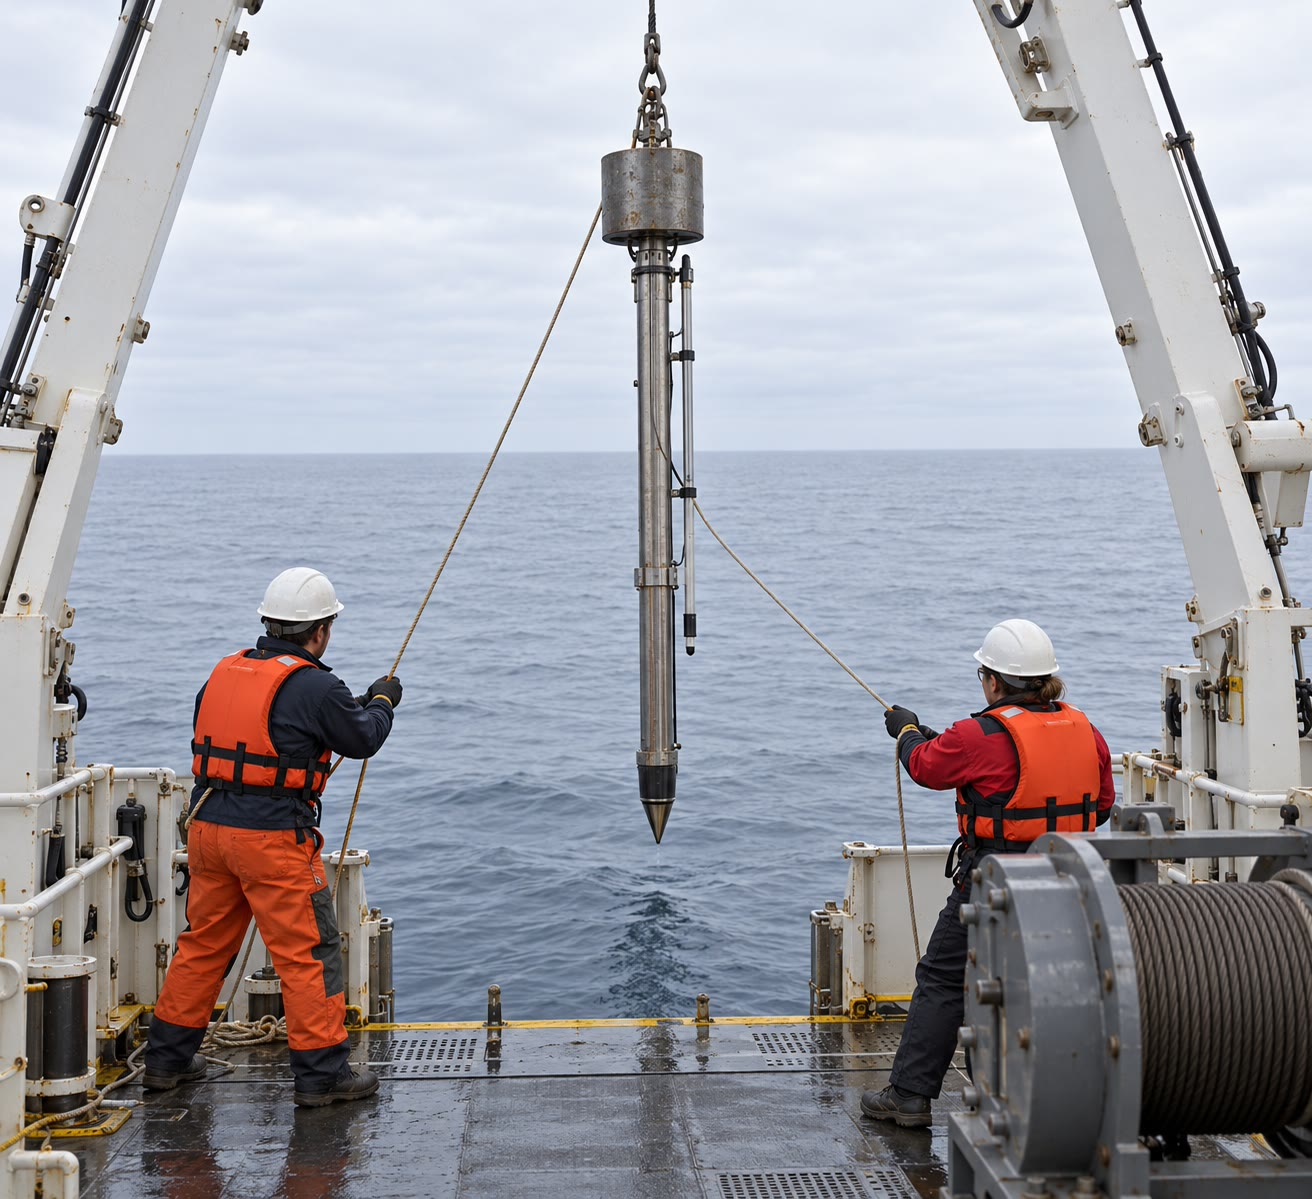
\includegraphics[width=\linewidth]{images/book5/ai/b3-heatflow-probe.jpg}

{\scriptsize एक ऊष्मा-प्रवाह भाला, जिसे शोध-पोत के पिछले भाग से नीचे उतारा जाने वाला है
(AI से बनाया गया चित्रण)।}
\end{minipage}
\end{inthefield}

\section{अभ्यास}

\begin{exercise}[$\star$]\label{exo:b3:lithosphere-thermal-models:1}
$\kappa = \qty{e-6}{m^2.s^{-1}}$ मानकर, चालन-समय $L^2/\kappa$
$L = 1$, 10 और \qty{100}{km} के लिए, मिलियन वर्षों में परिकलित कीजिए।
\end{exercise}

\begin{exercise}[$\star$]\label{exo:b3:lithosphere-thermal-models:2}
एक पर्वत-श्रेणी का \qty{1}{mm/yr} की दर से अपरदन होता है, और उसकी पूर्ति के लिए ऊपरी
\qty{30}{km} भूपर्पटी से चट्टान ऊपर उठती है। $\kappa = \qty{e-6}{m^2.s^{-1}}$ मानकर
पेक्ले संख्या परिकलित कीजिए। क्या उस पर्वत-श्रेणी का जियोथर्म
केवल चालन द्वारा परिकलित किया जा सकता है?
\end{exercise}

\begin{exercise}[$\star$]\label{exo:b3:lithosphere-thermal-models:3}
अर्ध-समष्टि मॉडल में ($T_0 = 0$, $T_m = \qty{1450}{\celsius}$, $\kappa =
\qty{0.8e-6}{m^2.s^{-1}}$), \qty{5}{Myr} पुराने समुद्र-तल के नीचे \qty{10}{km} की गहराई पर तापमान,
(\qty{1}{Myr} $= \qty{3.156e13}{s}$; $\operatorname{erf}
0.445 = 0.471$) परिकलित कीजिए।
\end{exercise}

\begin{exercise}[$\star$]\label{exo:b3:lithosphere-thermal-models:4}
$C_q = \qty{490}{mW.m^{-2}.Myr^{1/2}}$ मानकर, समुद्र-तल से होने वाला ऊष्मा-प्रवाह
1, 25 और \qty{100}{Myr} पुराने समुद्र-तल के लिए परिकलित कीजिए। इन तीनों में से
किसे संवेदक द्वारा सबसे अधिक कम आँके जाने की संभावना है?
\end{exercise}

\begin{exercise}[$\star\star$]\label{exo:b3:lithosphere-thermal-models:5}
अर्ध-समष्टि मॉडल में तापमान $T_m$ का \qty{90}{\percent} वहाँ पहुँचता है जहाँ
$\operatorname{erf}\eta = 0.9$, $\eta = 1.163$ है। $\kappa =
\qty{0.8e-6}{m^2.s^{-1}}$ मानकर, 10, 40 और \qty{100}{Myr} पर वह गहराई परिकलित कीजिए।
\end{exercise}

\begin{exercise}[$\star\star$]\label{exo:b3:lithosphere-thermal-models:6}
पाठ के मानों के साथ अर्ध-समष्टि मॉडल $C =
\qty{370.5}{m.Myr^{-1/2}}$ देता है। अन्य सभी मानों को यथावत रखते हुए, कितना तापीय प्रसार
गुणांक प्राप्त मान \qty{350}{m.Myr^{-1/2}} देगा? इसके बजाय कौन-सा अन्य प्राचल
बदला जा सकता है?
\end{exercise}

\begin{exercise}[$\star\star$]\label{exo:b3:lithosphere-thermal-models:7}
प्लेट मॉडल का अनंतस्पर्शी ऊष्मा-प्रवाह $kT_m/L$ के लिए, जहाँ $L =
\qty{95}{km}$, $T_m = \qty{1450}{\celsius}$ तथा $L = \qty{125}{km}$,
$T_m = \qty{1350}{\celsius}$ के लिए, दोनों में $k = \qty{3.1}{W.m^{-1}.K^{-1}}$ मानकर, अनंतस्पर्शी ऊष्मा-प्रवाह परिकलित कीजिए।
कौन-सा परिणाम $C_q/\sqrt t$ से परिकलित पुराने महासागरीय तल के ऊष्मा-प्रवाह के
\qty{150}{Myr} पर, $C_q = \qty{490}{mW.m^{-2}.Myr^{1/2}}$ के साथ, अधिक निकट है?
\end{exercise}

\begin{exercise}[$\star\star$]\label{exo:b3:lithosphere-thermal-models:8}
एक प्रांत में $q_0 = \qty{60}{mW.m^{-2}}$, $h_r = \qty{10}{km}$ और $A_0h_r =
0.4\,q_0$ है। $A_0$, $q_m$ और \qty{35}{km} गहराई पर मोहो का तापमान,
$k = \qty{2.5}{W.m^{-1}.K^{-1}}$ मानकर, परिकलित कीजिए।
\end{exercise}

\begin{exercise}[$\star\star$]\label{exo:b3:lithosphere-thermal-models:9}
एक ही प्रांत के दो ग्रेनाइट प्लूटॉन $q_0 = \qty{66}{mW.m^{-2}}$ देते हैं, जिनमें $A_0
= \qty{3.0}{\micro W.m^{-3}}$ है, और $q_0 = \qty{48}{mW.m^{-2}}$ के साथ $A_0 =
\qty{1.2}{\micro W.m^{-3}}$ है। मान लीजिए वे
\cref{prop:b3:lithosphere-thermal-models:exponential} की रेखा पर स्थित हैं, तो $h_r$ और $q_m$ परिकलित कीजिए।
\end{exercise}

\begin{exercise}[$\star\star\star$]\label{exo:b3:lithosphere-thermal-models:10}
(क) दिखाइए कि आयु 0 से $t$ के बीच समुद्र-तल से खोई गई ऊष्मा, प्रति
इकाई क्षेत्रफल, अर्ध-समष्टि मॉडल में $Q(t) = 2k(T_m - T_0)\sqrt{t/(\pi\kappa)}$ है।
(ख) दिखाइए कि अवधसान $d - d_r = \alpha Q/\bigl(c(\rho_m -
\rho_w)\bigr)$ है, जहाँ $c = k/(\rho_m\kappa)$ विशिष्ट ऊष्मा है। (ग) पाठ के मानों के साथ
\qty{40}{Myr} पर इसकी संख्यात्मक जाँच कीजिए।
\end{exercise}

\begin{exercise}[$\star\star\star$]\label{exo:b3:lithosphere-thermal-models:11}
पाठ के प्लेट मॉडल में ($\tau = \qty{36.2}{Myr}$, $\rho_m\alpha T_mL/
\bigl(2(\rho_m - \rho_w)\bigr) = \qty{3104}{m}$), केवल प्रथम फ़ूरिये पद से परिकलित गहराई
पूरी श्रेणी से मुख्यतः $n = 3$ पद के कारण अधिक है।
उस पद का आकार 1, 10 और \qty{20}{Myr} पर परिकलित कीजिए, और वह आयु
ज्ञात कीजिए, जिसके बाद केवल प्रथम पद श्रेणी से \qty{10}{m} के भीतर आ जाता है।
\end{exercise}

\begin{exercise}[$\star\star\star$]\label{exo:b3:lithosphere-thermal-models:12}
(क) दिखाइए कि \cref{prop:b3:lithosphere-thermal-models:exponential} के जियोथर्म में
$T(z) \approx q_mz/k + A_0h_r^2/k$ है, जब $z \gg h_r$ हो। (ख)
\qty{1300}{\celsius} समतापरेखा की गहराई, $q_0 = \qty{40}{mW.m^{-2}}$ के लिए, अभ्यास 8 के मानों सहित, निकालिए।
(ग) $q_m$ को कितना घटाना होगा, ताकि वह गहराई
\qty{250}{km} तक पहुँचे, जो क्रेटनों की तेज़ जड़ों की गहराई है?
\end{exercise}

\section{समस्या: कटक से चालीस मिलियन वर्ष दूर}

\begin{problem}[{सप्ताहांत समस्या --- अर्ध-समष्टि और प्लेट, एक काल्पनिक महासागर की
गहराई, और उसकी प्लेट की मोटाई}]
\label{pb:b3:lithosphere-thermal-models:1}
% values: calc/ch05.py; plate_cooling.py; honda04:gdh1, ps77:depth-age, data:b5-depth-age
मान लीजिए $T_0 = 0$, $T_m = \qty{1450}{\celsius}$, $\kappa =
\qty{0.8e-6}{m^2.s^{-1}}$, $k = \qty{3.1}{W.m^{-1}.K^{-1}}$, $\alpha =
\qty{3.1e-5}{K^{-1}}$, $\rho_m = \qty{3300}{kg.m^{-3}}$, $\rho_w =
\qty{1030}{kg.m^{-3}}$, \qty{2500}{m} गहरा एक कटक, और \qty{1}{Myr} $=
\qty{3.156e13}{s}$।

\medskip\noindent\textbf{भाग I --- अर्ध-समष्टि।}
\begin{enumerate}
  \item 10 और \qty{40}{Myr} पर $\sqrt{\kappa t}$ परिकलित कीजिए।
  \item दोनों आयुओं पर तल के नीचे \qty{20}{km} पर तापमान
        ($\operatorname{erf}0.6294 = 0.6266$, $\operatorname{erf}0.3147 =
        0.3437$) परिकलित कीजिए।
  \item \qty{1000}{\celsius} समतापरेखा वहाँ है जहाँ $\operatorname{erf}\eta =
        0.6897$, $\eta = 0.7174$। दोनों आयुओं पर इसकी गहराई परिकलित कीजिए, और
        वह आयु ज्ञात कीजिए, जिस पर यह \qty{60}{km} तक पहुँचती है।
  \item दोनों आयुओं पर ऊष्मा-प्रवाह, और $C_q$ परिकलित कीजिए।
  \item एक कटक प्रत्येक ओर \qty{25}{mm/yr} की दर से फैलता है। \qty{95}{km} की प्लेट की
        पेक्ले संख्या परिकलित कीजिए। प्रत्येक स्तंभ को अलग-अलग ठंडा किया जाना
        क्यों उचित हो सकता है?
  \item \qty{95}{km} के पार चालन-समय परिकलित कीजिए। यह
        \qty{150}{Myr} पुराने तल के अर्ध-समष्टि मॉडल के बारे में क्या कहता है?
\end{enumerate}

\medskip\noindent\textbf{भाग II --- अवधसान।}
\begin{enumerate}[resume]
  \item किसी स्तंभ की तापमान-न्यूनता को अवधसान में बदलने वाला समस्थिति-संतुलन,
        और अर्ध-समष्टि में समाकल को अनंत तक ले जाना क्यों उचित हो सकता है,
        यह स्मरण कीजिए।
  \item गहराई–आयु नियम का $C$, और 10 और
        \qty{40}{Myr} पर गहराइयाँ परिकलित कीजिए।
  \item 40 और \qty{45}{Myr} के बीच वास्तविक महासागरीय तल की माध्यिका गहराई
        \qty{4475}{m} है, असंशोधित।
        \qty{42.5}{Myr} पर मॉडल से तुलना कीजिए, और
        माध्यिका में वे क्या सम्मिलित हैं जिन्हें मॉडल छोड़ देता है, उनकी सूची बनाइए।
  \item $C$ कितना बदलेगा, यदि $T_m$ \qty{1350}{\celsius} हो?
        आरोपित \qty{350}{m.Myr^{-1/2}} से तुलना कीजिए।
  \item युवा तल पर मापे गए ऊष्मा-प्रवाह $C_q/\sqrt t$ से नीचे क्यों आते हैं?
\end{enumerate}

\medskip\noindent\textbf{भाग III --- प्लेट।} मान लीजिए $L = \qty{95}{km}$।
\begin{enumerate}[resume]
  \item $\tau$ और आयाम $\rho_m\alpha T_mL/\bigl(2(\rho_m -
        \rho_w)\bigr)$ परिकलित कीजिए।
  \item $n = 1$, 3 और 5 वाले पदों के साथ \qty{40}{Myr} पर गहराई परिकलित कीजिए।
  \item केवल पहला पद उससे कितना भिन्न है, और
        यह इतना कम क्यों है?
  \item अर्ध-समष्टि और प्लेट के बीच का अंतर 40 और
        \qty{50}{Myr} पर परिकलित कीजिए, और रैखिक अंतर्वेशन से वह आयु
        अनुमान लगाइए जिस पर यह \qty{100}{m} तक पहुँचता है।
  \item \qty{40}{Myr} पर प्लेट का ऊष्मा-प्रवाह, पदों
        $n = 1$ से 3 तक लेकर परिकलित कीजिए, और अर्ध-समष्टि से तुलना कीजिए।
  \item अनंतस्पर्शी गहराई और ऊष्मा-प्रवाह दीजिए।
\end{enumerate}

\medskip\noindent\textbf{भाग IV --- एक काल्पनिक महासागर।} एक काल्पनिक महासागर में, जिसका
कटक \qty{2500}{m} गहरा है; तल, अवसाद के लिए संशोधन के बाद
समुद्री पर्वतों और उभारों से दूर, \qty{120}{Myr} पर \qty{5700}{m} गहरा है और
\qty{40}{Myr} पर \qty{4800}{m}। प्लेट का $L$ अज्ञात है; अन्य हर मान
ऊपर के अनुसार है।
\begin{enumerate}[resume]
  \item केवल पहला फ़ूरिये पद रखकर गहराई
        \qty{120}{Myr} पर $L$ के फलन के रूप में, जिसमें $\tau$ स्वयं
        $L$ पर निर्भर है, लिखिए।
  \item पुनरावृत्ति द्वारा $L$ के लिए इसे हल कीजिए, $L = \qty{100}{km}$ से आरंभ करके:
        पहले $\tau$ परिकलित कीजिए, फिर \qty{5700}{m} से मेल खाने वाला $L$
        ज्ञात कीजिए जो उसी $\tau$ के साथ हो, और यह क्रम दोहराइए।
  \item प्राप्त $L$ से \qty{40}{Myr} पर गहराई परिकलित कीजिए, और
        अर्ध-समष्टि और मापी गई \qty{4800}{m} से तुलना कीजिए।
  \item $\tau$ परिकलित कीजिए, जो उस $L$ के लिए हो, और इस महासागर की अनंतस्पर्शी गहराई।
  \item किस आयु के बाद तल अपनी अनंतस्पर्शी गहराई से
        \qty{100}{m} के भीतर आ जाता है?
  \item काल्पनिक महासागर के पुराने तल से मेल खाने वाली प्लेट की मोटाई
        $L$ दीजिए।
\end{enumerate}
\end{problem}
